\documentclass[12pt,letterpaper]{article}

\usepackage[portrait]{geometry}
\geometry{tmargin=1in,bmargin=1in,lmargin=1in,rmargin=1in}
\usepackage{graphicx}
\usepackage{amsmath}
%\usepackage{../latex/lplfitch}
\usepackage{enumitem}
\usepackage{color}
\usepackage{tcolorbox}
\tcbuselibrary{skins}

\colorlet{xlightblue}{blue!5}

\newtcolorbox{beamerlikethm}[1]{
  title=#1,
  beamer,
  colback=xlightblue,
  colframe=blue!30,
  fonttitle=\textsc,
  left=1mm,
  right=1mm,
  top=1mm,
  bottom=1mm,
  middle=1mm
}

\usepackage{fancyvrb}
\usepackage{fancyhdr}
\pagestyle{fancy}

\lhead{\Large{\bf Problem Set 4: \textsc{Reductions}}}
\chead{}
\rhead{Due: Tuesday 11/23 11:59PM}
\lfoot{CS 375 - Analysis of Algorithms}
\cfoot{}
\rfoot{Page \thepage}
\renewcommand{\headrulewidth}{3pt}
\renewcommand{\footrulewidth}{3pt}

\usepackage{tikz}
\usetikzlibrary{automata,positioning}

\begin{document}
Feel free to work in groups of at most 4 for these - if you have a group of more than 4, please run it by me first. If you do work in a group, please include the names of those that you worked with. \textbf{However: each student should submit a separate copy where the solutions have been written by yourself.}

\begin{enumerate}
    \item (10 points) A certain table tennis league is organized so that each season the $n$ players play against each other in a round-robin format, so that each player plays against each other player. The player who wins the most games is declared the winner: ties are handled by tossing a coin. A certain player has come to us mid season, worrying that they may have been technically eliminated. Our goal is to determine in a polynomial amount of time whether they can still win or not. Show that you can solve this problem with a runtime that is polynomial in $n$. Specifically, I want a polynomial time reduction to the flow decision problem. With even more clarity: 
    \begin{beamerlikethm}{\textsc{Elimination Game (EG)}}
        \textbf{Input: }Players $P_1, ..., P_n$, where player $P_i$ has won $w_i$ games so far, and remaining games $G_1, ..., G_m$. \\
        \textbf{Output: }\textsc{True} if $P_n$ cannot possibly finish the most wins out of $P_1, ..., P_n$.
    \end{beamerlikethm} 
    \begin{beamerlikethm}{\textsc{Flow}}
        \textbf{Input: }A graph $G$ with special vertices $s$ and $t$, capacities $c_e$ for every edge $e$, and a number $k$.\\
        \textbf{Output: }\textsc{True} if there is a valid flow on $G$ with value $k$ and \textsc{False} otherwise.
    \end{beamerlikethm}
    For full credit for this problem, I'm asking you to show:  $\text{EG}\leq_p\textsc{Flow}$.
    
    As an example, suppose this league has 8 players $P_1, ..., P_8$, where we are trying to determine if $P_8$ has been eliminated. We are given that the only game left to be played is between $P_6$ and $P_7$.
    We are also given that $P_6$, $P_7$, and $P_8$ each have 5 wins in total. Then no matter the results of the remaining games (note that every game individually cannot end in a tie), $P_8$ cannot be the winner of the league.
    \item (10 points) Google has a list $A_1, ..., A_n$ of advertisers that want to show ads to a group of users $u_1, ..., u_m$. Specifically, each advertiser $A_i$ has a list of users $G_i$ (a subcollection of $u_1, ..., u_m$) that it would like to show ads to (these groups may overlap); however, different advertisers have purchased different plans from Google, so Google will only show $r_i$ users the advertisement from $A_i$. Additionally, Google has run some analytics over their userbase and knows for each $u_j$ the number $c_j$ of ads $u_j$ can see before $u_j$ will get fed up and install an adblock. Your goal is to determine whether Google can display ads so that $r_i$ of advertiser $A_i$'s ads get shown to users in $G_i$, no user $u_j$ gets more than $c_j$ ads, and no user gets shown the same ad multiple times. 
    \begin{beamerlikethm}{\textsc{Advertisement Problem (Ads)}}
        \textbf{Input: }Advertisers $A_1, ..., A_n$ and users $u_1, ..., u_m$, groups of users $G_1, ..., G_n$, numbers $r_1, ..., r_n$ and $c_1, .., c_m$\\
        \textbf{Output: }\textsc{True} if there is a way to show users ads so that each advertiser has its ads shown to $r_i$ users in $G_i$ and no user $u_j$ gets shown more than 1 ad from any particular advertiser and no more than $c_j$ ads in total and \textsc{False} otherwise.
    \end{beamerlikethm}
    Specifically, I'm asking you to show that $\textsc{Ads}\leq_p\textsc{Flow}$.
    \item I've mentioned a few times how decision problems are easier to conceptualize for reduction type problems rather than optimization, but it's good to check along the way that these problems really are the ``same'', at least in terms of difficulty. Let's check for the Clique problem:
    \begin{beamerlikethm}{\textsc{Clique Decision (CD)}}
        \textbf{Input: }A graph $G$ and number $k$ \\
        \textbf{Output: }\textsc{True} if there are $k$ vertices in $G$ that are all adjacent to each other and \textsc{False} otherwise. 
    \end{beamerlikethm}
    \begin{beamerlikethm}{\textsc{Clique Optimization (CO)}}
        \textbf{Input: }A graph $G$\\
        \textbf{Output: } The largest collection of vertices in $G$ that are all adjacent to each other. 
    \end{beamerlikethm}
    Show that 
    \begin{enumerate}
        \item (5 points) if you have a polynomial time algorithm for CO then you can design a polynomial time algorithm for CD
        \item (10 points) if you have a polynomial time algorithm for CD then you can design a polynomial time algorithm for CO
    \end{enumerate} 
    \item Often times we look at problems over graphs which we assume are either directed or undirected, but maybe we start wondering about which of these types of graphs are harder to deal with. Consider the following graph isomorphism problem: we are given two graphs, and we want to see if one is simply a relabeling of the other. For example, consider the following graphs:
    \begin{center}
        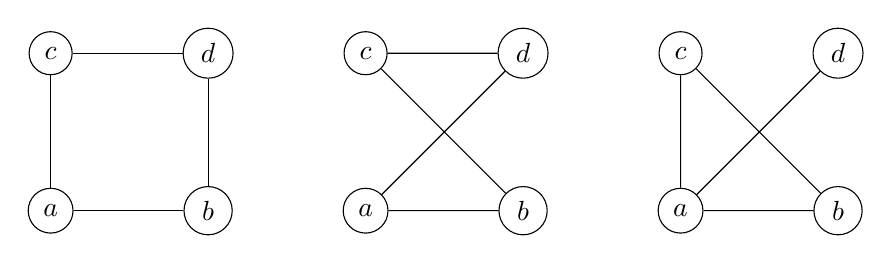
\begin{tikzpicture}
            \node[draw, circle] (a) at (0, 0) {$a$};
            \node[draw, circle] (b) at (2, 0) {$b$};
            \node[draw, circle] (c) at (0, 2) {$c$};
            \node[draw, circle] (d) at (2, 2) {$d$};
            \draw[-] (a) -- (b) -- (d) -- (c) -- (a) {};
            \node[draw, circle] (a) at (4, 0) {$a$};
            \node[draw, circle] (b) at (6, 0) {$b$};
            \node[draw, circle] (c) at (4, 2) {$c$};
            \node[draw, circle] (d) at (6, 2) {$d$};
            \draw[-] (a) -- (b) -- (c) -- (d) -- (a) {};
            \node[draw, circle] (a) at (8, 0) {$a$};
            \node[draw, circle] (b) at (10, 0) {$b$};
            \node[draw, circle] (c) at (8, 2) {$c$};
            \node[draw, circle] (d) at (10, 2) {$d$};
            \draw[-] (a) -- (b) -- (c) -- (a) -- (d) {};
        \end{tikzpicture}
    \end{center}
    The first two are just relabellings of the vertices, but there is no way to relabel the vertices of the last one to become the same as the first two.
    
    Let $n$ be the number of vertices and $m$ be the number of edges. 
    \begin{enumerate}
        \item (5 points) Show that if you have a $O(n+m)$ time algorithm for the graph isomorphism problem for directed graphs, then you can design a $O(n+m)$ time algorithm for the graph isomorphism problem on undirected graphs. 
        \item (10 points) Show that if you have a $O(n+m)$ time algorithm for the graph isomorphism problem for undirected graphs, then you can design a $O(n+m)$ time algorithm for the graph isomorphism problem on directed graphs. 
    \end{enumerate}
\end{enumerate}
\end{document}